%% ------------------------------------------------------------------------- %%n
\chapter{Descrição do Problema e Proposta}
\label{cap:Proposta}

O estudo da planctologia é de grande importância na comunidade científica, principalmente na oceanografia. O nome plâncton vem do Grego planktos e significa errante, que vaga ou flutua. Caracteriza-se, assim, por organismos planctônicos os que não possuem o poder de locomoção suficiente para evitar o transporte passivo pelas massas de água [\cite{calazans2011organismos}].  A importância do estudo dessas criaturas se dá não somente por serem responsáveis por cerca de 45\% do oxigênio produzido mundialmente [\cite{brierleyplankton}],  através da fotossíntese do fitoplâncton, mas também pela grande diversidade de classes e de características como forma, tamanho e até da natureza do local de coleta [\cite{calazans2011organismos}]. 

O plâncton é taxonomicamente diverso [\cite{brierleyplankton}]. Dentre os grupos temos o fitoplâncton (plantas), o zooplâncton (animais), o bacterioplâncton (bactérias e algas cianobactérias) e o virioplâncton (vírus aquáticos). Embora possam existir tamanhos maiores, a maioria deles são muito pequenos, variando de alguns micrômetros a 5 mm de comprimento. Além disso, existem muitas maneiras de classificar esses organismos, como em função do seu tamanho ou aspectos ecológicos [\cite{calazans2011organismos}].


A amostragem de criaturas marítimas é datada desde de 1829, quando Thompson utilizou uma rede para coletar larvas de crustáceos e de cracas [\cite{brierleyplankton}], mas foi Victor Hensen, em 1887, o primeiro pesquisador a desenvolver, de fato, um sistema para coleta de amostragens de plânctons de forma quantitativa [\cite{benfield2007rapid, wiebe2003hensen, allen1919contribution}]. Naquela época estavam interessados em responder três questões fundamentais: i) quais organismos planctônicos estão presentes no mar? ii) quantos de cada tipo estão presentes? e iii) como a composição dos plânctons muda com o passar do tempo?  [\cite{benfield2007rapid}]. Essas questões continuam atuais e graças ao avanço de sistemas e equipamentos de coleta, assim como de técnicas computacionais, há um grande esforço científico para responder à essas perguntas.


Hoje existem diversas maneiras de se fazer a amostragem de plânctons como, através de garrafas, redes, bombas de sucção e sistemas ópticos [\cite{calazans2011organismos}]. A figura ~\ref{fig:amostragem_planctons} mostra o exemplo de uma rede planctônica. É interessante notar que nos últimos anos houve uma proliferação em sistemas ópticos. Esses sistemas permitem, por exemplo, que algumas espécies de planctôns, por serem muitos delicadas, possam ter suas imagens capturadas, o que nem sempre é possível com outras técnicas [\cite{benfield2007rapid}].


\begin{figure}
  \centering
  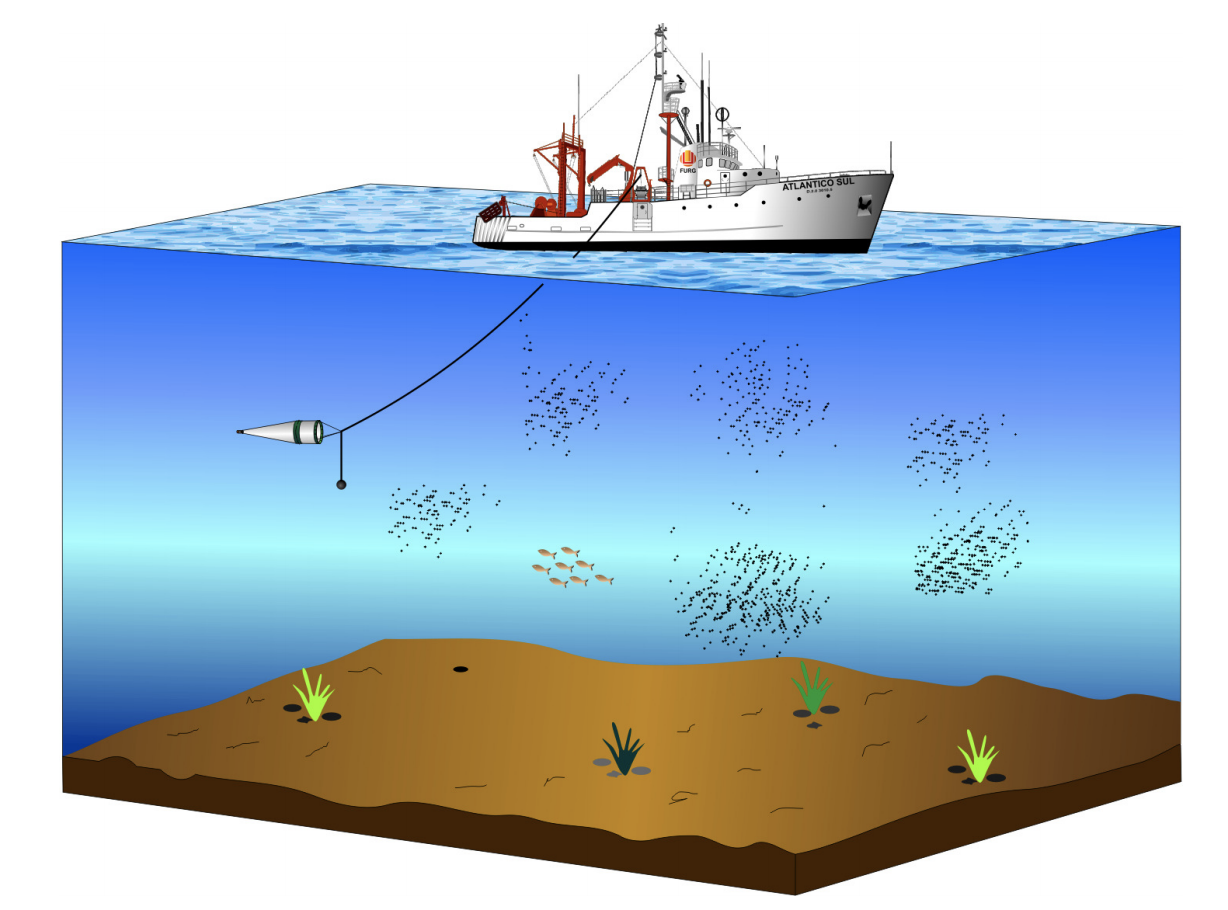
\includegraphics[width=.8\textwidth]{figures/amostragem_planctons.png}
  \caption{Rede Planctônica (Calazans, 2011)}
  \label{fig:amostragem_planctons}
\end{figure}



\section{Reconhecimento das classes de Plânctons}
\label{sec:reconhecimento_planctons}


Após a fase de coleta, especificamente através de sistemas ópticos, tem-se um conjunto de imagens de plânctons que não possuem rótulos. Essa categorização é importante pois é através dela que é possível utilizar do aprendizado computacional e gerar um classificador capaz de automatizar a rotulação de novas imagens. Esse é um problema antigo no caso dos plânctons [\cite{jeffries1980computer, jeffries1984automated, berman1990image, tang1998automatic}]   e ainda não totalmente resolvido[\cite{luo2003learning, davis2004real, grosjean2004enumeration, luo2005active, hu2005automatic, blaschko2005automatic, hu2006accurate, sosik2007automated, bell2008assessment, soh2008segmentation, al2016plankton, luo2017automated, al2018intelligent}].

O grande desafio é que demanda-se muito tempo e pessoas extremamente especializadas para cumprir essa tarefa, já que elas possuem, por exemplo, uma grande variedade de classes, formas e tamanhos. Como resultado, normalmente temos uma lacuna muito grande entre o tempo de coleta das imagens e a rotulação, assim como o possível erro humano na correta categorização das espécies. Somado a isso, muitas vezes, já temos um novo equipamento que possuem fotos com características diferentes das anteriores. Ou seja, apesar de todo o avanço que tivemos com equipamentos e técnicas, o problema de categorização persiste desde 1800, quando Thompson e Hensen iniciaram a coleta dessas criaturas [\cite{brierleyplankton, benfield2007rapid}]. 

É interessante notar que, caso tivéssemos todas as imagens com rótulos, nosso problema se reduziria em criar um classificador capaz de generalizar para as diversas taxonomias de plânctons possíveis. No entanto, nosso problema começa em um passo anterior: precisamos de dados rotulados para, então, pensarmos no classificador. É necessário, portanto, encontrar uma maneira de reduzir o esforço gasto na rotulação de amostras, obtendo, como resultado, um classificador de acurácia equivalente ou melhor do que uma abordagem padrão, com todos os dados rotulados. Como visto no capítulo dois, uma das abordagens conhecidas para isso é através do Aprendizado Ativo. 


\section{Aprendizado Ativo Integrado com o Conhecimento Humano Especializado}
\label{sec:aprendizado_ativo_conhecimento_humano}

O Aprendizado Ativo é uma abordagem interessante quando precisamos diminuir o esforço de rotulação e ainda gerarmos um classificador decente. Como visto no capítulo anterior, estudos recentes tentam incorporar o conhecimento humano nesse framework [\cite{castro2009human, kottke2018other}], sendo que uma maneira interessante de se fazer isso é através da interação do humano com a visualização de dados [\cite{yang2018visually, bernard2018comparing, weigl2016mapview}]. Além disso, no caso dos plânctons, estudos mostram que a incorporação de conhecimentos de especialistas aumenta a acurácia dos modelos [\cite{benfield2007rapid}].

A figura ~\ref{fig:frameworks_AL} à esquerda mostra o framework clássico do Aprendizado Ativo. Nele temos cinco passos, sendo: i) um conjunto de dados não rotulados. No inicio do ciclo de aprendizado ativo teremos apenas alguns exemplos com rótulo correto para que já exista uma primeira versão de um classificador, ii) através de uma função matemática o algoritmo selecionará as amostras que tem menos certeza das categorias, iii) o classificador categoriza as amostras, iv) o oráculo valida ou corrige e v) o classificador incorpora as amostras corretas para o treinamento. Após isso as fases se repetem até algum critério de parada.

\begin{figure}
  \centering
  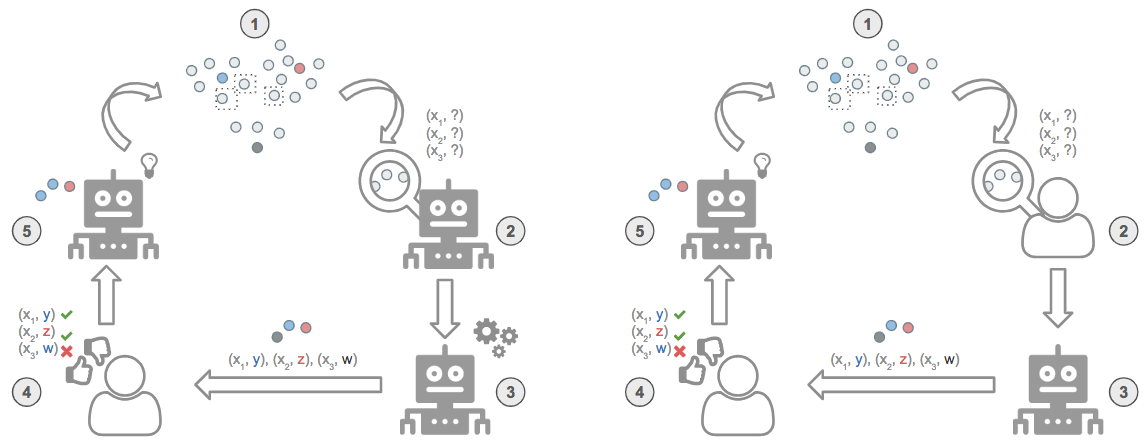
\includegraphics[width=0.95\textwidth]{figures/Frameworks_Active_Learning.png}
  \caption{esq: Framework Aprendizado Ativo Clássico, dir: Framework Aprendizado Ativo com Interação Humana na Seleção de Amostras}
  \label{fig:frameworks_AL}
\end{figure}

No caso do ciclo clássico, o oráculo serve apenas para validar as amostras do classificador. Como citado no capítulo fundamental teórico, essa atuação acaba fazendo com limitemos muito a atuação do especialista. Nossa proposta é fazer com que o oráculo seja, além de um validador, um selecionador de amostras [\cite{kottke2018other}]. A mesma figura à direita ilustra essa situação. A diferença é que no passo dois o oráculo também é responsável por selecionar os exemplos que considera mais representativo. 

A maneira pela qual será possível escolher os exemplos será através da projeção do espaço de features em um plano 2D, já que, geralmente, esse espaço possui uma alta dimensionalidade. O que queremos é encontrar uma transformação tal que $\mathcal{R}^d \xrightarrow{} \mathcal{R}^c$, com $c \ll d$ [\cite{van2009dimensionality}]. Será através dessa projeção que o especialista poderá selecionar os dados que ele acredita serem os mais representativos no ciclo para incorporar no ciclo de aprendizado ativo. 

%\section{Extração de Features}
%\label{sec:extracao_features}

%A extração de features será feita através de uma arquitetura de Deep Learning. 


%\section{Projeção do Espaço de Features}
%\label{sec:projecao_espaco_features}

\section{Base de Dados}
\label{sec:base_de_dados}

Neste trabalho teremos quatro bases de dados disponíveis. Todas 


\subsection{LAPS} 
\label{sec:basededados_laps}

Este dataset foi desenvolvido pelo LAPS,  (Laboratório de Sistemas Planctônicos do Departamento de Ocenanografia Biológica, do Instituto Ocenanogr[afico da Universidade de São Paulo]
XX classes de zooplanctons, onde todas as imagens são


\subsection{NDSB} 
\label{sec:basededados_ndsb}

% \cite{cowen2015planktonset}


\subsection{Japan} 
\label{sec:basededados_japan}



